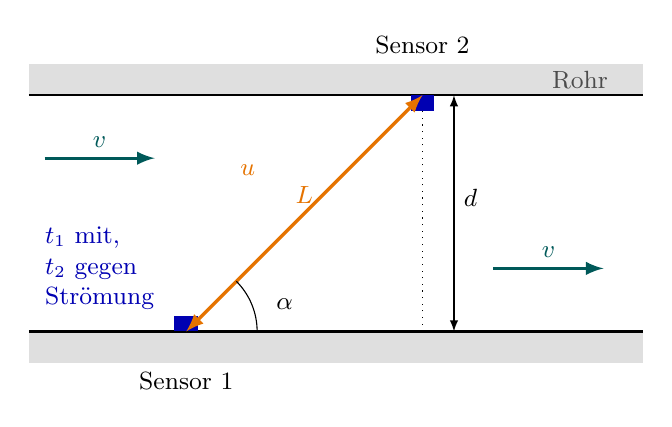
\begin{tikzpicture}[>=latex, x=1cm, y=1cm]
  % Rohrwand oben / unten
  \fill[gray!25] (-2,1.5) rectangle (5.8,1.9);
  \fill[gray!25] (-2,-1.9) rectangle (5.8,-1.5);
  \draw[thick] (-2,1.5) -- (5.8,1.5);
  \draw[thick] (-2,-1.5) -- (5.8,-1.5);
  \node[font=\small, gray!60!black] at (5.0,1.7) {Rohr};
  % Stroemung
  \draw[->, very thick, teal!70!black] (-1.8,0.7) -- (-0.4,0.7) node[midway, above, font=\small] {$v$};
  \draw[->, very thick, teal!70!black] (3.9,-0.7) -- (5.3,-0.7) node[midway, above, font=\small] {$v$};
  % Sensoren
  \fill[blue!70!black] (-0.15,-1.5) rectangle (0.15,-1.3);
  \fill[blue!70!black] (2.85,1.3) rectangle (3.15,1.5);
  \node[font=\small, below] at (0,-1.9) {Sensor 1};
  \node[font=\small, above] at (3,1.9) {Sensor 2};
  % Puls (hin und zurueck) auf der Strecke L
  \draw[<->, very thick, orange!90!black] (0,-1.5) -- (3,1.5);
  \node[font=\small, orange!90!black, sloped, above] at (1.5,0) {$L$};
  \node[font=\small, orange!90!black, left] at (1.0,0.55) {$u$};
  % Dreieck: Durchmesser d und Rohrachse
  \draw[dotted] (3,-1.5) -- (3,1.3);
  \draw[<->] (3.4,-1.5) -- (3.4,1.5);
  \node[font=\small, right] at (3.4,0.2) {$d$};
  % Winkel alpha zur Rohrachse
  \draw (0.9,-1.5) arc (0:45:0.9);
  \node[font=\small] at (1.25,-1.15) {$\alpha$};
  % Zeiten
  \node[font=\small, blue!70!black, align=left] at (-1.1,-0.7) {$t_1$ mit,\\$t_2$ gegen\\Strömung};
\end{tikzpicture}
